\section{Example 1: proton--$\Lambda$ from AO2D}

\begin{frame}{Example 1: proton--$\Lambda$ from AO2D}
 \begin{block}{Our goal}
 Produce a proton--$\Lambda$ correlation function, starting from an AO2D.
 \end{block}
 \begin{enumerate}
 \item \textbf{Part 1:} producer configuration for collisions, protons and $\Lambda$.
 \item \textbf{Part 2:} proton and $\Lambda$ QA.
 \item \textbf{Part 3:} proton--$\Lambda$ pairing and correlation.
 \end{enumerate}
 \medskip
 \textbf{Complete example files:} \texttt{examples/01-proton-lambda/}\par
 \small The final run script and configuration already contain every task; their settings evolve step by step during the live demonstration.
 \note{Instructor-led demonstrations, not exercises. This example implements the complete proton-Lambda chain, introduced through five live steps. The supplied input is a Run 3 pp data AO2D, LHC26ad, run 570703.}
 \src{O2Physics/PWGCF/Femto/TableProducer/femtoProducer.cxx; O2Physics/PWGCF/Femto/Tasks/femtoTrackQa.cxx}
\end{frame}


\begin{frame}[fragile]{Part 1: collision filters}
 \begin{lstlisting}
 "CollisionFilter": {
   "vtxZMin": "-10", "vtxZMax": "10",
   "multMin": "0",   "multMax": "5000",
   "centMin": "0",   "centMax": "100",
   "magFieldMin": "-5", "magFieldMax": "5"
 }
 \end{lstlisting}
 \begin{itemize}
 \item In this example the vertex range is $-10\leq z_{\rm vtx}\leq10$ cm; multiplicity and centrality bounds are broad.
 \item Magnetic-field bounds are in kG. Further options include sphericity and the MC sub-generator ID.
 \end{itemize}
 \note{The prefix is CollisionFilter, singular, unlike TrackFilters. This is an excerpt from the actual example configuration. The collision builder uses inclusive bounds. subGeneratorId=-1 disables that MC-specific filter. In normal production a failed collision filter prevents the event from entering the produced collision sample.}
 \src{O2Physics/PWGCF/Femto/Core/collisionBuilder.h}
\end{frame}

\begin{frame}[fragile]{Part 1: collision selection flags}
 \begin{lstlisting}
 "CollisionBits": {
   "passThrough": "false",
   "sel8": "-1",
   "rctFlags": "1",
   "noSameBunchPileup": "0"
 }
 \end{lstlisting}
 \small Integer settings control the role of these event-selection flags:
 \par\medskip
 \renewcommand{\arraystretch}{1.2}
 \begin{tabular}{cll}
 \toprule
 Value & Role & Producer behavior\\
 \midrule
 \texttt{"1"} & Minimal & Required; its guaranteed bit is omitted.\\
 \texttt{"-1"} & Optional & Stored as a bit; contributes to the optional OR.\\
 \texttt{"0"} & Disabled & Neither applied nor stored.\\
 \bottomrule
 \end{tabular}
 \par\medskip
 \small RCT is minimal; \texttt{sel8} is optional; \texttt{noSameBunchPileup} is disabled. The RCT quality definition is configured separately.
 \note{These are the boolean collision-flag settings, not the table-output auto/off/on switches. The optional OR follows the same BaseSelection rule described earlier. CollisionBits also supports vectors of occupancy/sphericity thresholds and trigger selections. hCollisionSelection records the metadata. CollisionBits.passThrough is separate from TrackBits.passThrough.}
 \src{O2Physics/PWGCF/Femto/Core/collisionBuilder.h; O2Physics/PWGCF/Femto/Core/baseSelection.h}
\end{frame}

\begin{frame}[fragile]{Part 1: RCT quality requirements}
 \begin{lstlisting}
 "CollisionBits": {"rctFlags": "1"},
 "CollisionRctFlags": {
   "label": "CBT_hadronPID",
   "useZdc": "false",
   "treatLimitedAcceptanceAsBad": "false"
 }
 \end{lstlisting}
 \small \texttt{CBT\_hadronPID} is our usual choice: it checks FT0, ITS, TPC tracking/PID and TOF quality.
 \begin{itemize}
 \item Other presets include \texttt{CBT}, \texttt{CBT\_electronPID}, \texttt{CBT\_calo}, \texttt{CBT\_muon} and \texttt{CBT\_muon\_glo}.
 \item \texttt{useZdc} additionally includes ZDC quality, relevant for Pb--Pb.
 \item We usually keep limited-acceptance periods when the limitation is reproducible in MC: \texttt{treatLimitedAcceptanceAsBad = "false"}.
 \end{itemize}
 \note{CollisionBits.rctFlags controls the selection role; CollisionRctFlags controls which RCT requirements are checked. The preset label selects a detector-quality combination, not a particle PID cut. In the example rctFlags=1 makes it minimal. The local RCTFlagsChecker defines the available preset labels.}
 \src{O2Physics/PWGCF/Femto/Core/collisionBuilder.h; O2Physics/Common/CCDB/RCTSelectionFlags.h}
\end{frame}

\begin{frame}[fragile]{Part 1: configurable trigger selections}
 \begin{lstlisting}
 "CollisionBits": {
   "triggers": {"values": ["triggerName1", "triggerName2"]},
   "triggerBcTolerance": "100"
 },
 "ConfCcdb": {"triggerPath": "EventFiltering/Zorro/"}
 \end{lstlisting}
 \small The names above are illustrative; the available trigger names depend on the production.
 \begin{itemize}
 \item Zorro provides one decision for each configured trigger, matched in bunch crossings within the configured tolerance.
 \item Trigger decisions are encoded as \textbf{equal-array} selections: one bit per trigger, each compared with \texttt{"1"}.
 \item Trigger decisions are \textbf{optional}: when they are the only optional selections, only events firing at least one configured trigger are stored.
 \end{itemize}
 \small The current example has an empty trigger list.
 \note{This is an illustrative trigger configuration, not a change to the supplied minimum-bias example. CollisionBits.triggers defaults to an empty vector. ConfCcdb.triggerPath selects the Zorro CCDB location, and triggerBcTolerance controls matching around the collision global BC. CutCulator shows the trigger names in the selection metadata. A consumer can explicitly require particular stored trigger bits; configuring optional triggers alongside sel8 does not require both.}
 \src{O2Physics/PWGCF/Femto/Core/collisionBuilder.h; O2Physics/PWGCF/Femto/Core/selectionContainer.h}
\end{frame}

\begin{frame}[fragile]{Part 1: minimal track-quality selections}
 \small In \texttt{examples/01-proton-lambda/configuration.json}, under \texttt{femto-producer}:
 \begin{lstlisting}
 "TrackFilters": {
   "ptMin": "0.3", "ptMax": "4.0",
   "etaMin": "-0.8", "etaMax": "0.8"
 },
 "TrackBits": {
   "tpcClustersMin":    {"values": ["90", "100", "110"]},
   "tpcCrossedRowsMin": {"values": ["80", "100", "110"]},
   "itsClustersMin":    {"values": ["5", "6"]},
   "itsIbClustersMin":  {"values": ["1"]}
 }
 \end{lstlisting}
 \begin{itemize}
 \item These quality observables are \textbf{minimal} selections in the builder.
 \item Every retained standalone track passes each loosest threshold.
 \item Tighter thresholds are recorded as bits for later working points.
 \end{itemize}
 \small The full configuration also includes DCA selections and shared-cluster limits.
 \note{The JSON on this slide is an excerpt, not a replacement for the complete configuration. The minimal/optional/neutral role is defined by addSelection in TrackSelection::configure. Changing the vector values does not change that role. TrackBits.passThrough remains false.}
 \src{O2Physics/PWGCF/Femto/Core/trackBuilder.h}
\end{frame}

\begin{frame}[fragile]{Part 1: proton PID optional, pion PID neutral}
 \begin{lstlisting}
 "requirePidProton": "true",
 "tpcProton":    {"values": ["-3;3", "-2.5;2.5"]},
 "tpctofProton": {"values": ["3.0", "2.5"]},
 "requirePidPion": "false",
 "tpcPion":      {"values": ["-3;3"]}
 \end{lstlisting}
 \begin{itemize}
 \item \texttt{requirePidProton = "true"}: configured proton PID decisions become \textbf{optional} selections for producer acceptance.
 \item \texttt{requirePidPion = "false"}: configured pion PID decisions remain \textbf{neutral}; pion PID cannot admit a track by itself.
 \item Retained proton candidates still carry the pion PID decision, so we can apply a pion veto later with a rejection mask.
 \end{itemize}
 \small The same \texttt{requirePid*} pattern exists for the other species.
 \note{Only proton requirePid is true in this example. The optional conditions are ORed in the producer, while minimal quality must all pass. Neutral does not mean the bit is a veto automatically: the consumer must explicitly put it in a rejectionMask. The local builder evaluates PID a second time for accepted tracks to populate competing-hypothesis bits. No pion rejection is applied in the initial QA run.}
 \src{O2Physics/PWGCF/Femto/Core/trackBuilder.h}
\end{frame}

\begin{frame}[fragile]{Part 1: set the TOF threshold already in the producer}
 \begin{lstlisting}
 # Producer: TrackBits
 "minMomTofProton": "0.75"
 # Consumer: TrackSelection1
 "pidThres": "0.75"
 \end{lstlisting}
 \begin{itemize}
 \item Below $p=0.75$ GeV/$c$: proton PID can use TPC information.
 \item At and above the producer threshold: a track without TOF cannot pass the proton optional selections.
 \item Rejecting these tracks before storing them reduces the derived-data size.
 \end{itemize}
 \begin{block}{The consumer can choose a lower threshold}
 All configured PID decisions are evaluated for retained candidates, so the consumer's \texttt{pidThres} can also be lower than the producer's \texttt{minMomTofProton}.
 \end{block}
 \note{These are total-momentum thresholds, not transverse momentum. In the local implementation the producer gate uses p >= threshold, while the consumer uses the low mask at p <= pidThres. TOF presence alone does not impose a combined PID cut: the example QA consumer explicitly requires the TPCTOF bit at high momentum. With only requirePidProton enabled, another species cannot rescue a high-p track without TOF. If additional optional species are enabled, their acceptance can change which tracks survive.}
 \src{O2Physics/PWGCF/Femto/Core/trackBuilder.h; O2Physics/PWGCF/Femto/Core/partitions.h}
\end{frame}

\begin{frame}[fragile]{Part 1: $\Lambda$ filters}
 \begin{lstlisting}
 "V0Filters": {
   "ptMin": "0.3", "ptMax": "6",
   "etaMin": "-0.8", "etaMax": "0.8",
   "massMinLambda": "1.08", "massMaxLambda": "1.16"
 }
 \end{lstlisting}
 \begin{itemize}
 \item V0 candidates are reconstructed from a pair of oppositely charged daughter tracks.
 \item The filters define the candidate kinematic acceptance and a broad $\Lambda$ mass window.
 \item Topology, daughter quality and daughter PID are handled by \texttt{LambdaBits}.
 \end{itemize}
 \note{Candidate filters use the Lambda mass hypothesis. Daughter-index dependencies require the track table even without standalone-track QA. The process-function choices are explained on their own slide after the selection configuration.}
 \src{O2Physics/PWGCF/Femto/TableProducer/femtoProducer.cxx; O2Physics/PWGCF/Femto/Core/v0Builder.h}
\end{frame}

\begin{frame}[fragile]{Part 1: $\Lambda$ selection bits and K$^0_{\rm S}$ rejection}
 \begin{lstlisting}
 "LambdaBits": {
   "cpaMin":          {"values": ["0.99", "0.995"]},
   "dcaDauMax":       {"values": ["1.5", "1.0"]},
   "dauTpcClustersMin": {"values": ["80"]},
   "posDauTpcProton": {"values": ["5", "3"]},
   "negDauTpcPion":   {"values": ["5", "3"]},
   "rejectK0shortMassRanges": {"values": ["0.475;0.515"]}
 }
 \end{lstlisting}
 \small For $\Lambda\to p\pi^-$, the daughters follow the proton and pion hypotheses. The K$^0_{\rm S}$ rejection instead tests their reconstructed $\pi^+\pi^-$ mass: candidates inside $0.475$--$0.515$ GeV/$c^2$ are rejected.
 \begin{block}{No K$^0_{\rm S}$ rejection}
 \texttt{"rejectK0shortMassRanges": \{"values": [";"]\}}\par
 A plain \texttt{";"} means no excluded mass range: every candidate passes this rejection selection.
 \end{block}
 \note{These selections are minimal in normal production. The configured K0short rejection decision passes when the candidate lies outside the excluded mass interval. The current one-entry rejection range is the guaranteed minimal baseline and carries no stored bit; tighter configured alternatives can carry bits. Replacing its only range by ";" disables rejection without changing the four tighter bits used by the example's mask 15. The full JSON also includes daughter eta/DCA, radius and decay-vertex selections.}
 \src{O2Physics/PWGCF/Femto/Core/v0Builder.h; O2Physics/PWGCF/Femto/Core/selectionContainer.h}
\end{frame}

\begin{frame}{Part 1: open-ended acceptance and rejection ranges}
 \small Ranges have the form \texttt{"lower;upper"}. Either limit may be omitted.
 \medskip
 \footnotesize
 \renewcommand{\arraystretch}{1.1}
 \begin{tabular}{p{.14\textwidth}p{.37\textwidth}p{.39\textwidth}}
 \toprule
 Bounds & Acceptance: TPC PID & Rejection: competing mass $m$\\
 \midrule
 Both & \texttt{"-3;3"}\newline accepts $-3\leq n\sigma\leq3$ & \texttt{"0.475;0.515"}\newline rejects $0.475\leq m\leq0.515$\\
 Upper only & \texttt{";3"}\newline accepts $n\sigma\leq3$ & \texttt{";0.515"}\newline rejects $m\leq0.515$\\
 Lower only & \texttt{"-3;"}\newline accepts $n\sigma\geq-3$ & \texttt{"0.475;"}\newline rejects $m\geq0.475$\\
 Neither & \texttt{";"}\newline accepts every value & \texttt{";"}\newline rejects no value\\
 \bottomrule
 \end{tabular}
 \medskip
 \small
 \begin{block}{The meaning depends on the selection type}
 Acceptance tests \textbf{inside} the range; rejection tests \textbf{outside}. With \texttt{";"}, every value passes either selection.
 \end{block}
 \note{Acceptance corresponds to kInsideRange and rejection to kOutsideRange. Nonempty bounds are inclusive for the accepted/excluded interval; the outside decision is strict. Missing lower/upper bounds extend to minus/plus infinity in the conceptual description. The completely open rejection range ";" is a deliberate special case in parseRangeString: it denotes reject nothing, rather than excluding the entire real line. This table describes the individual selection decision, independent of its minimal/optional/neutral role. Mass values are in GeV/c2.}
 \src{O2Physics/PWGCF/Femto/Core/selectionContainer.h}
\end{frame}

\begin{frame}[fragile]{Part 1: TOF PID for $\Lambda$ daughters}
 \begin{lstlisting}
 "LambdaBits": {
   "posDauTofProton": {"values": ["5", "3"]},
   "negDauTofPion":   {"values": ["5", "3"]},
   "requireTof": "true",
   "keepTracksWithoutTof": "true"
 }
 \end{lstlisting}
 \begin{itemize}
 \item \texttt{requireTof}: makes the configured daughter TOF cuts mandatory.
 \item \texttt{keepTracksWithoutTof}: keeps daughters without a TOF signal.
 \end{itemize}
 \begin{block}{With a TOF signal}
 A measured TOF value that fails the mandatory cut still rejects the candidate.
 \end{block}
 \note{Illustrative extension, not enabled in the supplied baseline JSON: adding TOF thresholds can change mask assignments, which must be recomputed with CutCulator. With requireTof false, the TOF decisions are neutral and do not reject candidates at producer level; consumers may still select their bits. For anti-Lambda the positive daughter uses the pion hypothesis and the negative daughter the proton hypothesis. keepTracksWithoutTof overrides missing-signal failure only, not an actually measured PID failure.}
 \src{O2Physics/PWGCF/Femto/Core/v0Builder.h}
\end{frame}

\begin{frame}[fragile]{Part 1: producer process functions}
 \small
 \begin{lstlisting}
 "femto-producer": {
   "processTracksRun3pp": "false",
   "processTracksV0sRun3pp": "true"
 }
 \end{lstlisting}
 \begin{itemize}
 \item The process function defines the \textbf{data subscriptions}. Track-only processing subscribes to track inputs, without V0, cascade, kink or photon candidates.
 \item Processes handling V0s, cascades, kinks or photons require the corresponding input tables and builder/helper tasks in the analysis chain.
 \item The current producer has \textbf{no Run 2 process functions}. Run 3 variants cover pp and Pb--Pb, with data and MC options.
 \end{itemize}
 \begin{block}{Run 3 systems: the centrality estimator}
 pp uses \textbf{FT0M}; Pb--Pb uses \textbf{FT0C}.
 \end{block}
 \note{Track-only means only the track candidate category: the process also needs collision, event-selection, multiplicity and PID inputs. Process signatures determine subscriptions and therefore which upstream builders are needed; output-table switches alone do not activate candidate processing. The main pp/PbPb distinction discussed here is the centrality estimator stored by CollisionSelection::setCentrality: FT0M for kPP_Run3, FT0C for kPbPb_Run3. The local producer currently exposes Run 3 processing functions only. The final supplied configuration enables processTracksV0sRun3pp and disables processTracksRun3pp and the other producer processes.}
 \src{O2Physics/PWGCF/Femto/TableProducer/femtoProducer.cxx; O2Physics/PWGCF/Femto/Core/collisionBuilder.h}
\end{frame}

\begin{frame}[fragile]{Part 2: track QA -- particle and kinematic selections}
 \small Under \texttt{femto-track-qa}:
 \begin{lstlisting}
 "TrackSelection1": {
   "pdgCodeAbs": "2212", "chargeSign": "1", "chargeAbs": "1",
   "ptMin": "0.3", "ptMax": "4.0",
   "etaMin": "-0.8", "etaMax": "0.8",
   "phiMin": "0", "phiMax": "6.28318548"
 }
 \end{lstlisting}
 \begin{itemize}
 \item \texttt{chargeAbs}: rescales stored $p_{\mathrm T}/|Z|$ to physical momentum; \texttt{"2"} for $^3$He, usually \texttt{"1"}.
 \item \texttt{chargeSign}: \texttt{"1"} positive, \texttt{"-1"} negative, \texttt{"0"} both.
 \item \texttt{pdgCodeAbs}: supplies the four-vector mass for every species; PID is selected separately by masks.
 \end{itemize}
 \begin{block}{Antiparticles}
 \footnotesize Antiproton: \texttt{"chargeSign": "-1"}; \texttt{pdgCodeAbs} stays \texttt{"2212"}.
 \end{block}
 \note{The same mass-hypothesis principle applies to tracks and composite particle species. The stored track quantity is signedPt; physical pT is abs(chargeAbs*signedPt), while its sign identifies the track charge. The example selects positive protons with the shown kinematic bounds. The standard partition uses strict kinematic comparisons. These consumer selections can narrow the producer's sample but cannot recover discarded candidates. processData remains true in the full QA configuration.}
 \src{O2Physics/PWGCF/Femto/Core/trackBuilder.h; O2Physics/PWGCF/Femto/Core/partitions.h}
\end{frame}

\begin{frame}[fragile]{Part 2: track QA -- PID threshold and selection masks}
 \small Under \texttt{femto-track-qa.TrackSelection1}:
 \begin{lstlisting}
 "pidThres": "0.75",
 "maskLowMomentum": "64",
 "maskHighMomentum": "256"
 \end{lstlisting}
 \renewcommand{\arraystretch}{1.4}
 \begin{tabular}{lll}
 \toprule
 Total momentum & Required mask & Selection in this example\\
 \midrule
 $p\leq0.75$ GeV/$c$ & \texttt{"64"} & TPC proton PID: $-3\leq n\sigma_{\rm TPC,p}\leq3$\\
 $p>0.75$ GeV/$c$ & \texttt{"256"} & Combined TPC+TOF proton PID $\leq3$\\
 \bottomrule
 \end{tabular}
 \par\medskip
 \begin{itemize}
 \item \texttt{pidThres} refers to \textbf{total momentum}, not $p_{\mathrm T}$.
 \item Each mask requires all its selected bits; quality and PID decisions can be combined in the same mask.
 \item Here the producer already guarantees the baseline track quality; the masks add proton PID.
 \end{itemize}
 \note{The mask values are specific to the supplied normal-production configuration and were verified from producer metadata. The combined cut uses sqrt(nsigmaTPC squared + nsigmaTOF squared). CutCulator computes the values for the desired working point. Rejection masks are zero in the example, so no competing-species veto is applied. At exactly p=pidThres the local consumer uses the low mask. All rows selected by the kinematic partition must also satisfy the corresponding mask.}
 \src{O2Physics/PWGCF/Femto/Core/trackBuilder.h; O2Physics/PWGCF/Femto/Core/partitions.h}
\end{frame}

\begin{frame}[fragile]{Part 2: $\Lambda$ QA}
 \begin{lstlisting}
 "femto-v0-qa": {
   "processLambda": "true",
   "LambdaSelection1": {
     "pdgCodeAbs": "3122", "sign": "1",
     "massMin": "1.11", "massMax": "1.12",
     "mask": "15"
   }
 }
 \end{lstlisting}
 \begin{itemize}
 \item $\Lambda$ QA uses \texttt{LambdaSelection1}: candidate kinematics, mass window and selection mask.
 \item The QA distributions show the resulting particle samples and daughter observables.
 \end{itemize}
 \note{The live demonstration first shows proton QA, then adds Lambda QA after configuring the V0 producer. Here mask 15 requires cpaMin 0.995, daughter DCA 1.0 cm and both daughter TPC PID thresholds of 3. The four bit positions were verified locally. The candidate signal window is narrower than the producer mass window.}
 \src{O2Physics/PWGCF/Femto/Tasks/femtoTrackQa.cxx; O2Physics/PWGCF/Femto/Tasks/femtoV0Qa.cxx}
\end{frame}


\begin{frame}[fragile]{Part 2: where the QA histograms live}
 \begin{columns}[T]
 \begin{column}{.49\textwidth}
 \begin{block}{\texttt{AnalysisResults.root}}
 \begin{lstlisting}
femto-track-qa/
  Collision/...
  TrackQA/
    Analysis/  hPt, hEta, hPhi, ...
    QA/        track quality, DCA, ...
    PID/       detector PID, ...
    FitVars/   DCA distributions

femto-v0-qa/
  LambdaQA/
    Analysis/  kinematics, mass, ...
    QA/        topology, mass, ...
    FitVars/   pointing angle
 \end{lstlisting}
 \end{block}
 \end{column}
 \begin{column}{.47\textwidth}
 \small
 \begin{itemize}
 \item One top-level directory per task instance (or wagon).
 \item \texttt{Analysis/}: particle sample after the consumer selections.
 \item \texttt{QA/} and \texttt{PID/}: detailed observables enabled by the QA configuration.
 \item Daughter-track distributions accompany the $\Lambda$ sample.
 \end{itemize}
 \medskip
 \texttt{TrackBinning1} controls kinematics; \texttt{TrackQaBinning1} controls detailed QA and PID axes.
 \end{column}
 \end{columns}
 \note{This is a schematic directory layout, not a screenshot. Only booked histograms appear. FitVars purity histograms are deliberately skipped in full track QA because the full detector PID plots are already present. MC adds MC truth and origin templates.}
 \src{O2Physics/PWGCF/Femto/Core/trackHistManager.h; O2Physics/PWGCF/Femto/Core/v0HistManager.h}
\end{frame}

\begin{frame}[fragile]{Part 2: the binning belongs to the configuration}
 \begin{columns}[T]
 \begin{column}{.49\textwidth}
 \begin{lstlisting}
"TrackBinning1": {
  "pt": {"values": ["120", "0", "6"]}
},
"TrackQaBinning1": {
  "plot2d": "true",
  "plotProtonPid": "true",
  "momentumType": "1",
  "p": {"values": ["120", "0", "6"]},
  "tpcProton": {
    "values": ["200", "-10", "10"]
  },
  "dcaXy": {
    "values": ["200", "-0.2", "0.2"]
  }
}
 \end{lstlisting}
 \end{column}
 \begin{column}{.47\textwidth}
 \small
 \begin{block}{Uniform or variable-width axes}
 \texttt{["120", "0", "6"]}: 120 bins between 0 and 6.\par\medskip
 \texttt{["0", "0.3", "0.5", "1", "2", "4"]}: variable-width edges; first entry \texttt{"0"} is the marker.
 \end{block}
 \texttt{momentumType}: \texttt{"0"} $p_{\rm T}$, \texttt{"1"} $p$ at PV, \texttt{"2"} $p$ at TPC inner wall.\par\medskip
 $\Lambda$ equivalents: \texttt{LambdaBinning1}, \texttt{LambdaQaBinning1}; daughter axes have their own groups.
 \end{column}
 \end{columns}
 \note{Axes are shared wherever the same observable is used: pt changes both hPt and the pt axis of related multidimensional histograms. A binning change does not change a selection. plot2d and per-species plot flags control booking and memory. Values in the supplied JSON are all strings.}
 \src{O2Physics/PWGCF/Femto/Core/trackHistManager.h; O2Physics/PWGCF/Femto/Core/v0HistManager.h}
\end{frame}

\begin{frame}[fragile]{Part 3: proton--$\Lambda$ pair configuration}
 \begin{lstlisting}
"processLambdaSameEvent": "true", "processLambdaMixedEvent": "true",
"TrackSelection1": {
  "pdgCodeAbs": "2212", "chargeSign": "1", "pidThres": "0.75",
  "maskLowMomentum": "64", "maskHighMomentum": "256"
},
"LambdaSelection1": {
  "pdgCodeAbs": "3122", "sign": "1", "mask": "15",
  "massMin": "1.11", "massMax": "1.12"
},
"TrackBinning1":  {"pt": {"values": ["120", "0", "6"]}},
"LambdaBinning1": {"pt": {"values": ["120", "0", "6"]}},
"PairBinning":   {"kstar": {"values": ["600", "0", "6"]}}
 \end{lstlisting}
 \small Particle selections match QA; particle and pair histograms have separate binning groups.
 \note{Snippets show configurable groups within femto-pair-track-v0. The full consumer kinematic selections match the QA samples in the supplied JSON. Binning values illustrate configurable histogram axes and do not change cuts. Ordinary mixing is introduced first; tagging is added later. The prepared final configuration already enables tagging. sameSpecies is essential for identical-particle tasks using one shared selection; it is false for this cross-species task.}
 \src{O2Physics/PWGCF/Femto/Tasks/femtoPairTrackV0.cxx; O2Physics/PWGCF/Femto/Core/pairBuilder.h}
\end{frame}

\begin{frame}[fragile]{Part 3: event mixing}
 \footnotesize
 \begin{lstlisting}[basicstyle=\ttfamily\fontsize{7}{8}\selectfont]
"Mixing": {
  "policy": "0", "depth": "5", "eventStride": "1",
  "vtxBins": {"values": ["0", "-10", "0", "10"]},
  "multBins": {"values": ["0", "0", "50", "200"]},
  "enableEventMixingQa": "true", "enablePairCorrelationQa": "true"
}
 \end{lstlisting}
 \begin{columns}[T]
 \begin{column}{.48\textwidth}
 \begin{tabular}{cl}
 \toprule
 \texttt{policy} & Pool dimensions\\\midrule
 \texttt{"0"} & $z_{\rm vtx}$ + multiplicity\\
 \texttt{"1"} & $z_{\rm vtx}$ + centrality\\
 \texttt{"2"} & $z_{\rm vtx}$ + both\\
 \texttt{"3"} & $z_{\rm vtx}$ + centrality + $\Psi$*\\\bottomrule
 \end{tabular}
 \par\smallskip
 *Needs a supporting process; here: 0--2.
 \end{column}
 \begin{column}{.48\textwidth}
 \textbf{Depth 5:} up to five partners per anchor, in the same pool and dataframe.\par\smallskip
 \textbf{Stride:} keep \texttt{1}; increase only if processing time is too large. Larger values skip anchor windows.\par\smallskip
 \textbf{Bins:} leading \texttt{0} marks variable-width edges. Other axes: \texttt{centBins}, \texttt{eventPlaneAngle}.\par\smallskip
 \textbf{QA:} window sizes, event-property and particle-count correlations.
 \end{column}
 \end{columns}
 \begin{beamercolorbox}[sep=1mm,wd=\textwidth]{block body}
 \footnotesize\textbf{Identical particles:} \texttt{sameSpecies = true} avoids counting both $(i,j)$ and $(j,i)$ in SE. Proton--$\Lambda$: \texttt{false}.
 \end{beamercolorbox}
 \note{depth is a maximum; sparse pools, dataframe edges and pair acceptance reduce effective partners. Stride skips anchor windows, not tracks or all potential partner events. enableEventMixingQa books window-size and event-property QA; enablePairCorrelationQa books particle-count correlations. First vector entry 0 marks variable-width binning, whereas a positive first entry sets the number of uniform bins. This snippet illustrates stride 2; the prepared baseline uses stride 1. sameSpecies is explained on this mixing slide. Additional controls retained in the complete JSON: particleBinning sets the particle-count axis; seed randomizes identical roles (negative off, zero time-based, positive fixed). centBins and eventPlaneAngle accept the same ConfigurableAxis format as the shown axes.}
 \src{O2Physics/PWGCF/Femto/Core/pairHistManager.h; O2Physics/PWGCF/Femto/Core/pairProcessHelpers.h}
\end{frame}

\begin{frame}[fragile]{Part 3: the collision tagger}
 \begin{lstlisting}
"femto-producer-collision-tagger": {"processTrackLambda": "true"},
"femto-pair-track-v0": {
  "processLambdaSameEvent": "true",
  "processLambdaMixedEvent": "false",
  "processLambdaMixedEventWithTagging": "true"
}
 \end{lstlisting}
 \begin{itemize}
 \item \textbf{Recommended: always include the collision tagger} in pair workflows. It reads the wagons' particle selections.
 \item One tag bit per wagon and pair type: for proton--$\Lambda$, the collision contains at least one selected proton \emph{and} one selected $\Lambda$.
 \item The pair task discovers its own bit automatically and filters its mixed-event pool using \texttt{FColTags}.
 \item Empty candidate pools are avoided; pair cleaning and CPR still apply.
 \end{itemize}
 \note{Tagging changes the eligible mixing pool: both species must exist in each tagged collision. It is not merely a cache for the untagged mixed-event definition. Tags are recomputed when consumer selections change and are not persisted by our producer-only example. Do not manually set TaggingTrackLambdaPair.internalTagMask. The tagger must be present in the same workflow, with processTrackLambda enabled.}
 \src{O2Physics/PWGCF/Femto/TableProducer/femtoProducerCollisionTagger.cxx; O2Physics/PWGCF/Femto/Core/collisionTagger.h}
\end{frame}

\begin{frame}{Part 3: event mixing illustrated}
 \small\textbf{Example: selected pool A}\quad $-2\leq z_{\rm vtx}<0$ cm, $20\leq N<24$.\par
 We have \textbf{100 events in this pool}.\par\smallskip
 \begin{columns}[T]
 \begin{column}{.47\textwidth}
 \centering\textbf{Depth 10, stride 5}\par\smallskip
 \begin{tikzpicture}[x=.024cm,y=.024cm,every node/.style={font=\scriptsize}]
 \fill[pale] (0,0) rectangle (100,-100);
 \foreach \row in {0,...,98} {
   \pgfmathtruncatemacro{\last}{min(100,\row+11)}
   \fill[gray!35] (\row+1,-\row) rectangle (\last,-\row-1);
 }
 \foreach \row in {0,5,...,95} {
 \pgfmathtruncatemacro{\last}{min(100,\row+11)}
 \fill[teal!75] (\row+1,-\row) rectangle (\last,-\row-1);
}
 \foreach \tick in {0,20,...,100} {
   \draw[gray!30,line width=.2pt] (\tick,0)--(\tick,-100);
   \draw[gray!30,line width=.2pt] (0,-\tick)--(100,-\tick);
 }
 \draw[gray] (0,0) rectangle (100,-100);
 \node[above] at (50,4) {100 partner events};
 \node[rotate=90] at (-9,-50) {100 anchor events};
\end{tikzpicture}
 \par\smallskip
 \textcolor{teal}{193 event pairs}\par
 \footnotesize Every fifth anchor window; skipped windows are grey.
 \end{column}
 \begin{column}{.47\textwidth}
 \centering\textbf{Depth 10, stride 1}\par\smallskip
 \begin{tikzpicture}[x=.024cm,y=.024cm,every node/.style={font=\scriptsize}]
 \fill[pale] (0,0) rectangle (100,-100);
 \foreach \row in {0,...,98} {
   \pgfmathtruncatemacro{\last}{min(100,\row+11)}
   \fill[teal!75] (\row+1,-\row) rectangle (\last,-\row-1);
 }
 
 \foreach \tick in {0,20,...,100} {
   \draw[gray!30,line width=.2pt] (\tick,0)--(\tick,-100);
   \draw[gray!30,line width=.2pt] (0,-\tick)--(100,-\tick);
 }
 \draw[gray] (0,0) rectangle (100,-100);
 \node[above] at (50,4) {100 partner events};
 \node[rotate=90] at (-9,-50) {100 anchor events};
\end{tikzpicture}
 \par\smallskip
 \textcolor{teal}{945 event pairs}\par
 \footnotesize Every anchor, with up to ten partner events.
 \end{column}
 \end{columns}
 \par\smallskip
 \footnotesize Mixing runs to the pool edge: the last anchor windows contain \textbf{fewer than 10 partner events}.\par\smallskip
 Stride 5 reduces event pairs by about 80\%. Events from different pools never mix.
 \note{Schematic selfCombinations ordering within one dataframe and pool. Depth 10 produces sum(min(10,99-i),i=0..98)=945 event pairs. Stride 5 retains anchor windows i=0,5,...,95, yielding 18*10+9+4=193 event pairs. Grey cells are eligible depth-10 event pairs whose anchor window is skipped. No individual events are labelled; coarse grid lines are visual guides every 20 events. Actual selection, field consistency and valid particle-pair acceptance can lower effective counts.}
 \src{O2Physics/PWGCF/Femto/Core/pairProcessHelpers.h; O2Physics/PWGCF/Femto/Core/pairHistManager.h}
\end{frame}

\begin{frame}[fragile]{Part 3: close-pair rejection}
 \begin{columns}[T]
 \begin{column}{.48\textwidth}
 \begin{lstlisting}
"CprTrackV0Daughter": {
  "cutAverage": "false",
  "cutAnyRadius": "true",
  "cutElipsoidal": "true",
  "detaMax": "0.01",
  "dphistarMax": "0.01",
  "detaCenter": "0",
  "dphistarCenter": "0"
}
 \end{lstlisting}
 \small For proton--$\Lambda$, the primary track is compared with the charged daughters.\par\medskip
 Both cut switches \texttt{"false"} disable CPR.
 \end{column}
 \begin{column}{.48\textwidth}
 \centering
 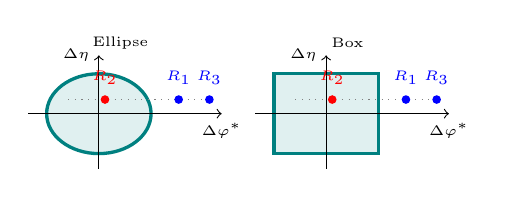
\begin{tikzpicture}[scale=.78,every node/.style={font=\tiny}]
 \foreach \offset/\shape in {0/Ellipse,1/Box} {
   \begin{scope}[shift={(3.7*\offset,0)}]
     \node at (.35,1.15) {\shape};
     \ifnum\offset=0\relax
       \fill[teal!12] (0,0) ellipse (.85 and .65);
       \draw[teal,very thick] (0,0) ellipse (.85 and .65);
     \else
       \fill[teal!12] (-.85,-.65) rectangle (.85,.65);
       \draw[teal,very thick] (-.85,-.65) rectangle (.85,.65);
     \fi
     \draw[->] (-1.15,0)--(2.0,0) node[below] {$\Delta\varphi^*$};
     \draw[->] (0,-.9)--(0,.95) node[left] {$\Delta\eta$};
     \draw[dotted,gray] (-.5,.23)--(1.8,.23);
     \fill[red] (.1,.23) circle (2pt) node[above=2pt] {$R_2$};
     \fill[blue] (1.3,.23) circle (2pt) node[above=2pt] {$R_1$};
     \fill[blue] (1.8,.23) circle (2pt) node[above=2pt] {$R_3$};
   \end{scope}
 }
 \end{tikzpicture}
 \par\smallskip
 \footnotesize One radius ($R_2$) lies inside the cut: \texttt{cutAnyRadius = true} rejects the pair.\par\medskip
 \texttt{cutAverage}: tests the average $\Delta\varphi^*$ over radii.\par\medskip
 \texttt{cutElipsoidal = true}: ellipse.\par
 \texttt{cutElipsoidal = false}: box.\par\smallskip
 The cut can be off-centre: set \texttt{detaCenter} and \texttt{dphistarCenter}.
 \end{column}
 \end{columns}
 \src{O2Physics/PWGCF/Femto/Core/closePairRejection.h}
\end{frame}

\begin{frame}{Part 3: all CPR diagnostic options}
 \footnotesize
 \renewcommand{\arraystretch}{1.08}
 \begin{tabular}{p{.42\textwidth}p{.52\textwidth}}
 \toprule
 \texttt{CprTrackV0Daughter} option & Purpose\\\midrule
 \texttt{plotAllRadii}, \texttt{plotAverage} & $\Delta\eta$--$\Delta\varphi^*$ at each radius / averaged.\\
 \texttt{plotAngularCorrelation} & $\eta_1$ vs $\eta_2$, $\varphi_1$ vs $\varphi_2$.\\
 \texttt{plotKinematic} & Distribution of blocked pairs.\\
 \texttt{kinematicVariable} & \texttt{"0"}: $k^*$, \texttt{"1"}: $k_{\rm T}$, \texttt{"2"}: $m_{\rm T}$, \texttt{"3"}: $Q_3$.\\
 \texttt{kinematicMin}, \texttt{kinematicMax} & Kinematic window for plotting; negative disables a bound.\\
 \texttt{binningKinematic} & Axis of blocked-pair kinematics.\\
 \texttt{binningDeta}, \texttt{binningDphistar} & Close-pair QA axes.\\
 \texttt{binningCorrelationPhi}, \texttt{binningCorrelationEta} & Angular-correlation QA axes.\\
 \texttt{seed} & Role randomization: negative off, zero time-based, positive fixed.\\
 \texttt{magField} & Field in kG for pure generator-level MC; reco uses collision field.\\\bottomrule
 \end{tabular}
 \src{O2Physics/PWGCF/Femto/Core/closePairRejection.h}
\end{frame}

\begin{frame}[fragile]{Part 3: pair cleaning and pair cuts}
 \begin{block}{A track cannot be paired with its own $\Lambda$}
 The cleaner rejects a primary-track candidate when its stored track index matches either $\Lambda$ daughter index. This check is automatic; there is no activation flag for shared-track cleaning.
 \end{block}
 \begin{columns}[T]
 \begin{column}{.48\textwidth}
 \begin{lstlisting}
"PairCuts": {
  "kstarMin": "-1", "kstarMax": "-1",
  "ktMin": "-1", "ktMax": "-1",
  "mtMin": "-1", "mtMax": "-1",
  "massInvMin": "-1", "massInvMax": "-1",
  "mixOnlyCommonAncestor": "false",
  "mixOnlyNonCommonAncestor": "false",
  "useMotherAsAncestor": "false",
  "kinematicVariable": "0"
}
 \end{lstlisting}
 \end{column}
 \begin{column}{.48\textwidth}
 \small Negative pair-kinematic bounds are disabled.\par\medskip
 In MC, ancestry can require common or non-common ancestry (mutually exclusive); \texttt{useMotherAsAncestor} chooses direct mother instead of partonic mother.\par\medskip
 \texttt{PairCuts.kinematicVariable} selects the kinematic variable: $k^*$, $k_{\rm T}$ or $m_{\rm T}$.\par\smallskip
 \texttt{PairCleanerBinning.kinematic} sets its histogram binning for blocked pairs.
 \end{column}
 \end{columns}
 \src{O2Physics/PWGCF/Femto/Core/pairCleaner.h; O2Physics/PWGCF/Femto/Core/pairHistManager.h}
\end{frame}

\begin{frame}[fragile]{Part 3: which ancestor is compared?}
 \begin{lstlisting}
"femto-producer": {
  "MonteCarlo": {"findLastPartonicMother": "true"}
}
 \end{lstlisting}
 \begin{itemize}
 \item \texttt{true}: first parton after the initial collision, before reaching a beam particle when tracing backwards.
 \item \texttt{false}: last parton before hadronization, closest to the final-state hadron.
 \end{itemize}
 \begin{block}{Producer choice, consumer comparison}
 \small The producer stores the chosen partonic ancestor. With \texttt{useMotherAsAncestor = false}, common/non-common checks compare these stored ancestors.\par\smallskip
 \texttt{useMotherAsAncestor = true} instead compares the direct mothers.
 \end{block}
 \note{The findLastPartonicMother name refers to backwards traversal: true follows the ancestry back towards the beam and retains the earliest parton after the initial collision. False selects the nearest partonic ancestor before hadronization. Both choices are partons, not a hadron before hadronization. The setting belongs to the producer MonteCarlo group and cannot be changed retrospectively by a consumer reading derived MC tables. Common and non-common requirements remain mutually exclusive.}
 \src{O2Physics/PWGCF/Femto/Core/mcBuilder.h; O2Physics/PWGCF/Femto/Core/pairCleaner.h}
\end{frame}



\begin{frame}{Part 3: mixing without collision tagging}
 \centering
 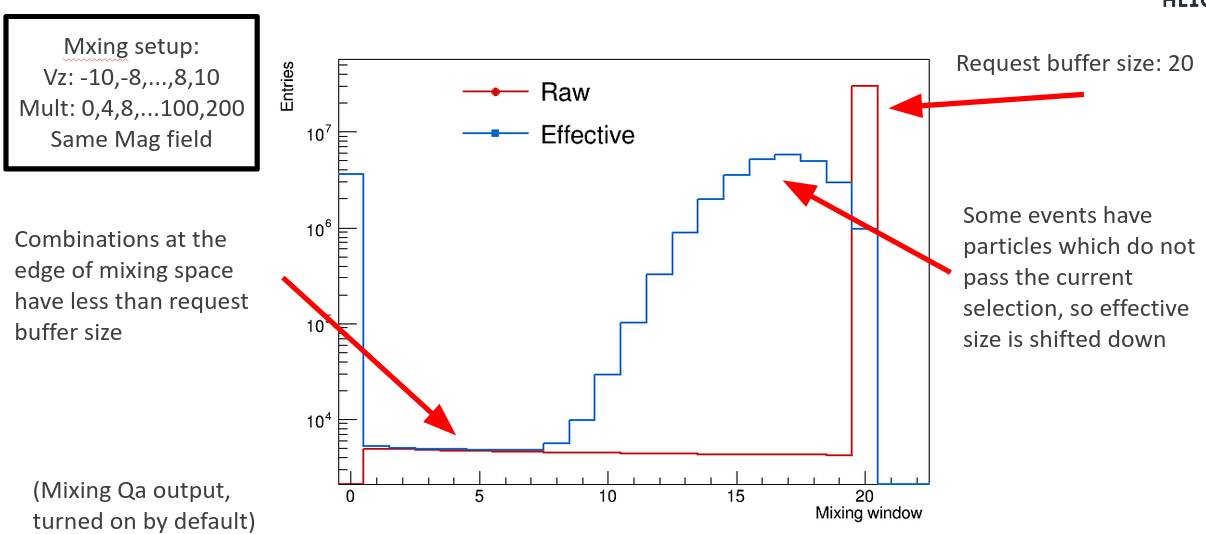
\includegraphics[width=\textwidth,height=.76\textheight,keepaspectratio]{slides/assets/mixing-without-tagging.png}
 \note{User-provided screenshot from another presentation. Raw windows reach the requested depth, apart from boundaries; effective windows lose partners without suitable selected candidates. The screenshot's statement that mixing QA is on by default refers to its original setup: in this checkout enableEventMixingQa defaults to false, and our demonstration explicitly enables it.}
 \src{O2Physics/PWGCF/Femto/Core/pairHistManager.h; O2Physics/PWGCF/Femto/Core/pairProcessHelpers.h}
\end{frame}

\begin{frame}{Part 3: mixing with collision tagging}
 \centering
 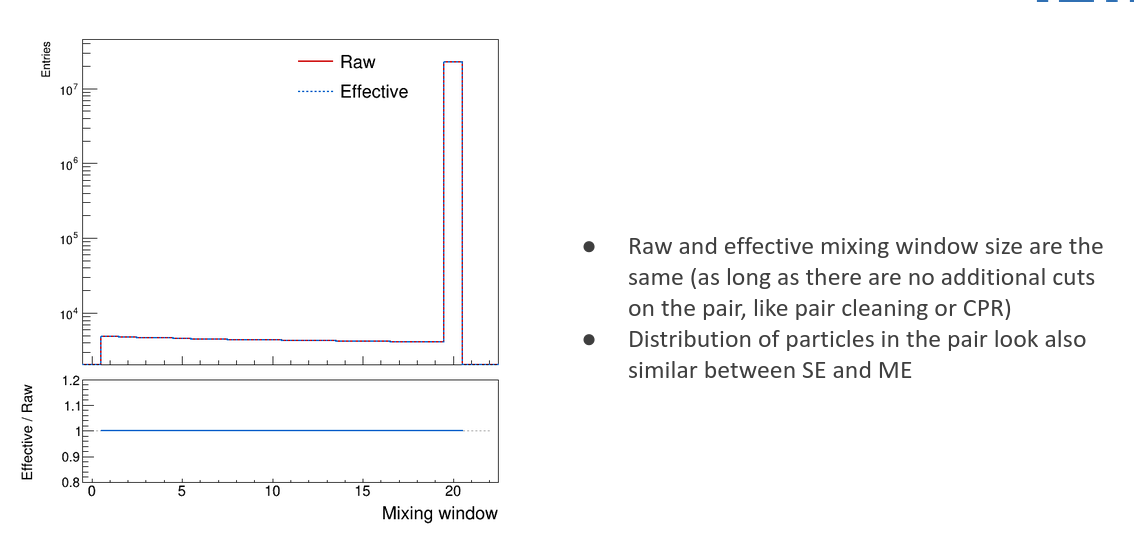
\includegraphics[width=\textwidth,height=.76\textheight,keepaspectratio]{slides/assets/mixing-with-tagging.png}
 \note{User-provided screenshot from another presentation. Tagging retains collisions containing the configured candidate species, so raw and effective mixing-window sizes can agree. Subsequent pair cleaning, CPR and pair cuts can still remove every candidate pair for a partner event, reducing the effective window. The screenshot is illustrative, not an output generated by the tutorial scripts.}
 \src{O2Physics/PWGCF/Femto/TableProducer/femtoProducerCollisionTagger.cxx; O2Physics/PWGCF/Femto/Core/pairProcessHelpers.h}
\end{frame}

\begin{frame}[fragile]{Part 3: pair histograms and dimensions}
 \begin{columns}[T]
 \begin{column}{.43\textwidth}
 \begin{lstlisting}[basicstyle=\ttfamily\fontsize{7}{8}\selectfont]
femto-pair-track-v0/
  TrackV0/
    SE/Analysis/...
    ME/Analysis/...
  TrackV0Cleaner/
    SE/...
    ME/...
  CPR_TrackV0Dau/
    SE/...
    ME/...
 \end{lstlisting}
 \small Same- and mixed-event pair distributions, shared-track cleaning and close-pair rejection QA.
 \end{column}
 \begin{column}{.53\textwidth}
 \begin{lstlisting}[basicstyle=\ttfamily\fontsize{7}{8}\selectfont]
"PairBinning": {
  "plotKstarVsMtVsMult": "false",
  "plotKstarVsMtVsMultVsCent": "true",
  "kstar": {"values": ["600", "0", "6"]},
  "mt": {"values": ["100", "1", "6"]},
  "multiplicity": {"values": ["1", "0", "5000"]},
  "centrality": {"values": ["1", "0", "100"]}
}
 \end{lstlisting}
 \small Plot switches turn higher-dimensional histograms on or off.
 \end{column}
 \end{columns}
 \par
 \small\textbf{Reuse a higher-dimensional THnSparse:} set unused dimensions to one bin covering their full range. No extra bin multiplicity in these axes; no separate histogram implementation for every axis combination.
 \note{The example enables hKstarVsMtVsMultVsCent and makes multiplicity and centrality inclusive via one bin, leaving differential kstar and mt axes. Use ranges covering the complete selected sample and handle underflow/overflow consistently in projections. Higher-dimensional sparse histograms allocate populated bins rather than the full Cartesian grid. Extra axes still have small coordinate/metadata overhead, so this is not a claim of literally zero memory/CPU cost. Basic 1D/2D pair histograms are TH1F/TH2F, not THnSparse; the reuse argument here applies to the higher-dimensional THnSparse plots. The histogram choices shown are illustrative and do not alter the runnable baseline configuration.}
 \src{O2Physics/PWGCF/Femto/Core/pairHistManager.h; O2Physics/PWGCF/Femto/Core/pairCleaner.h; O2Physics/PWGCF/Femto/Core/closePairRejection.h}
\end{frame}

\begin{frame}[fragile]{Part 3: single-particle histograms in the pair task}
 \begin{lstlisting}
femto-pair-track-v0/
  Track1/SE/Analysis/...     Track1/ME/Analysis/...
  Lambda1/SE/Analysis/...    Lambda1/ME/Analysis/...
 \end{lstlisting}
 \begin{columns}[T]
 \begin{column}{.48\textwidth}
 \begin{block}{Same event (SE)}
 \small Filled only when the collision contributes at least one valid pair.\par\medskip
 Each selected particle is filled \textbf{once per collision}, even if the collision contains several valid pairs.
 \end{block}
 \end{column}
 \begin{column}{.48\textwidth}
 \begin{block}{Mixed event (ME)}
 \small Filled for every valid mixed-event pair.\par\medskip
 A particle is filled \textbf{as many times as it is used} in accepted mixed-event pairs.
 \end{block}
 \end{column}
 \end{columns}
 \medskip
 \small SE and ME therefore retain their different particle-sampling weights.
 \note{Valid means after particle cleaning, shared-track pair cleaning, CPR and pair cuts. For SE, once any pair is accepted, the task loops over the selected particle slices and fills each particle that passes the particle cleaner once. Thus the SE constituent sample includes all selected cleaner-passing particles in a contributing collision, not only the unique constituents of accepted pairs. ME fills constituents inside the accepted-pair loop, so repeated uses carry repeated weight. The same distinction applies to single-particle FitVars histograms discussed later. Run scripts and local/Hyperloop instructions remain in the example directory for the live demonstration.}
 \src{O2Physics/PWGCF/Femto/Core/pairProcessHelpers.h; O2Physics/PWGCF/Femto/Core/pairBuilder.h}
\end{frame}
